\subsection{Tuần 1}

\subsubsection{Nội dung công việc: Tìm hiểu về công ty, môi trường làm việc, quy trình phát triển sản phẩm và định hướng thực tập.}
\textbf{Hoạt động:}
\begin{itemize}
    \item Tham gia chương trình định hướng thực tập, tìm hiểu về lịch sử hình thành, cơ cấu tổ chức và lĩnh vực hoạt động của công ty.
    
    \item Tìm hiểu môi trường làm việc, quy định nội bộ, quy trình làm việc và văn hóa doanh nghiệp.
    
    \item Nghiên cứu tổng quan về quản lý dự án trong lĩnh vực công nghệ thông tin.
    
    \item Tìm hiểu mô hình quản lý dự án theo chuẩn CMMI được áp dụng tại công ty.
    
    \item Nghiên cứu các giai đoạn trong vòng đời quản lý dự án bao gồm: khởi động, xác định yêu cầu, lập giải pháp, xây dựng, triển khai và kết thúc dự án.
    
    \item Tìm hiểu quy trình hoạch định dự án, xác định phạm vi công việc, lập kế hoạch nguồn lực và tiến độ thực hiện.
    
    \item Tìm hiểu cơ cấu tổ chức nhân sự trong dự án và vai trò của các thành viên tham gia dự án.
    
    \item Nghiên cứu mô hình làm việc Agile Scrum và cách tổ chức đội dự án theo Scrum Team.
    
    \item Tìm hiểu vai trò của Product Owner, Scrum Master và Development Team trong quá trình phát triển sản phẩm.
    
    \item Tìm hiểu các hoạt động quản lý yêu cầu khách hàng và quy trình phối hợp giữa khách hàng với đội dự án.
    
    \item Nghiên cứu quy trình quản lý thay đổi yêu cầu trong quá trình thực hiện dự án.
    
    \item Tìm hiểu quy trình quản lý rủi ro và các biện pháp giảm thiểu rủi ro trong dự án phần mềm.
    
    \item Tìm hiểu các hoạt động đảm bảo chất lượng (Quality Assurance) và kiểm thử phần mềm.
    
    \item Tìm hiểu quy trình triển khai hệ thống, hỗ trợ khách hàng, nghiệm thu và bàn giao sản phẩm.
    
    \item Tìm hiểu chính sách bảo hành, bảo trì và hỗ trợ sau triển khai của doanh nghiệp.
    
    \item Tìm hiểu tổng quan về dự án thực tập, nghiệp vụ của dự án và các công nghệ dự kiến được sử dụng trong quá trình thực hiện.
\end{itemize}
\subsubsection{Nội dung tìm hiểu và kiến thức thu nhận}

\paragraph{1. Tổng quan về quản lý dự án}

Quản lý dự án (Project Management) là quá trình áp dụng kiến thức, kỹ năng, công cụ và kỹ thuật nhằm lập kế hoạch, tổ chức, giám sát và kiểm soát các hoạt động của dự án để đạt được các mục tiêu đã đề ra. Trong lĩnh vực công nghệ thông tin, quản lý dự án đóng vai trò quan trọng trong việc đảm bảo sản phẩm được phát triển đúng phạm vi, đáp ứng yêu cầu khách hàng, hoàn thành đúng tiến độ và tối ưu chi phí thực hiện.

Một dự án phần mềm thường phải cân bằng giữa ba yếu tố chính gồm phạm vi công việc (Scope), thời gian thực hiện (Time) và chi phí (Cost). Bên cạnh đó, chất lượng sản phẩm (Quality) cũng là một yếu tố quan trọng quyết định sự thành công của dự án. Do đó, các doanh nghiệp thường xây dựng những quy trình quản lý chặt chẽ nhằm giảm thiểu rủi ro và nâng cao hiệu quả triển khai dự án.

\paragraph{2. Quy trình quản lý dự án theo chuẩn CMMI}

\begin{figure}[h]
    \centering
    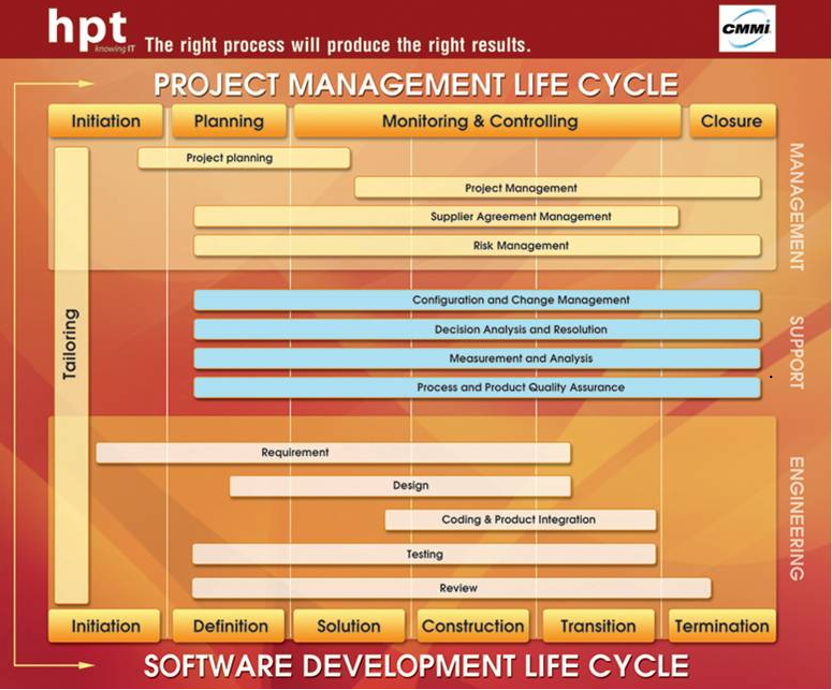
\includegraphics[width=0.8\textwidth]{include/image/cmmi.png}
    \caption{Quy trình CMMI cho phát triển phần mềm}
    \label{fig:cmmi}
\end{figure}

Qua quá trình tìm hiểu, công ty áp dụng mô hình CMMI (Capability Maturity Model Integration) trong quản lý và triển khai dự án phần mềm. Đây là một mô hình cải tiến quy trình được sử dụng rộng rãi trong ngành công nghệ thông tin nhằm chuẩn hóa hoạt động quản lý, nâng cao chất lượng sản phẩm và tăng khả năng thành công của dự án.

Theo mô hình này, dự án được chia thành nhiều giai đoạn với các mục tiêu, sản phẩm đầu ra và tiêu chí đánh giá cụ thể. Mỗi giai đoạn đều phải được xem xét, đánh giá và phê duyệt trước khi chuyển sang giai đoạn tiếp theo nhằm đảm bảo chất lượng của toàn bộ dự án.

\subparagraph{Giai đoạn khởi động}

Đây là giai đoạn đầu tiên của dự án, có nhiệm vụ xác định mục tiêu, phạm vi và tính khả thi của dự án. Các hoạt động chính bao gồm khảo sát nhu cầu khách hàng, xác định phạm vi công việc, ước lượng nguồn lực, xây dựng kế hoạch sơ bộ và ban hành quyết định khởi động dự án.

Kết quả của giai đoạn này là một kế hoạch tổng quan giúp các bên liên quan có được cái nhìn chung về mục tiêu và định hướng thực hiện dự án.

\subparagraph{Giai đoạn xác định yêu cầu}

Mục tiêu của giai đoạn này là thu thập, phân tích và làm rõ các yêu cầu từ khách hàng. Các yêu cầu được chuyển đổi thành các tài liệu đặc tả giúp đội phát triển hiểu rõ chức năng và đặc điểm của hệ thống cần xây dựng.

Trong quá trình này, các chuyên gia nghiệp vụ và phân tích hệ thống sẽ phối hợp với khách hàng để làm rõ các yêu cầu chức năng, yêu cầu phi chức năng, tiêu chí nghiệm thu và các ràng buộc của dự án. Đây là một trong những giai đoạn quan trọng nhất vì các sai sót trong việc xác định yêu cầu có thể ảnh hưởng đến toàn bộ quá trình phát triển sau này.

\subparagraph{Giai đoạn lập giải pháp}

Sau khi các yêu cầu được xác nhận, nhóm dự án tiến hành xây dựng các giải pháp kỹ thuật phù hợp. Công việc chính bao gồm thiết kế kiến trúc hệ thống, xác định các thành phần phần mềm, cơ sở dữ liệu, giao diện và các cơ chế tích hợp giữa các hệ thống.

Giai đoạn này giúp chuyển đổi các yêu cầu nghiệp vụ thành các giải pháp kỹ thuật cụ thể, đồng thời đánh giá tính khả thi của hệ thống trước khi tiến hành phát triển.

\subparagraph{Giai đoạn xây dựng}

Đây là giai đoạn hiện thực hóa các thiết kế thành sản phẩm phần mềm hoàn chỉnh. Các lập trình viên tiến hành phát triển các chức năng theo tài liệu thiết kế, đồng thời thực hiện kiểm thử đơn vị và kiểm thử tích hợp nhằm phát hiện sớm các lỗi phát sinh.

Bên cạnh hoạt động lập trình, các hoạt động kiểm thử và kiểm soát chất lượng cũng được thực hiện liên tục nhằm đảm bảo sản phẩm đáp ứng các tiêu chuẩn kỹ thuật đã đề ra.

\subparagraph{Giai đoạn triển khai}

Sau khi sản phẩm hoàn thiện và đạt yêu cầu chất lượng, hệ thống được triển khai lên môi trường thực tế. Các hoạt động chính bao gồm cài đặt hệ thống, cấu hình môi trường vận hành, hỗ trợ kiểm thử nghiệm thu và đào tạo người sử dụng.

Mục tiêu của giai đoạn này là đảm bảo khách hàng có thể sử dụng hệ thống một cách hiệu quả và ổn định trong môi trường thực tế.

\subparagraph{Giai đoạn kết thúc}

Giai đoạn kết thúc được thực hiện sau khi khách hàng hoàn thành việc nghiệm thu sản phẩm. Các tài liệu dự án, mã nguồn và các sản phẩm liên quan được tổng hợp và bàn giao cho bộ phận quản lý hoặc khách hàng theo quy định.

Ngoài ra, các bài học kinh nghiệm, phản hồi từ khách hàng và các chỉ số chất lượng cũng được thu thập nhằm phục vụ cho việc cải tiến quy trình và triển khai các dự án trong tương lai.

\paragraph{3. Hoạch định dự án}

Hoạch định dự án là hoạt động quan trọng nhằm xác định phương án triển khai dự án trước khi bắt đầu thực hiện. Nội dung hoạch định bao gồm xác định phạm vi công việc, phân chia nhiệm vụ, ước lượng nguồn lực, xây dựng kế hoạch tiến độ và xác định các mốc quan trọng của dự án.

Thông qua hoạt động hoạch định, nhóm dự án có thể dự đoán trước các khó khăn có thể phát sinh, phân bổ nguồn lực hợp lý và xây dựng các phương án ứng phó với rủi ro. Một kế hoạch tốt sẽ giúp tăng khả năng hoàn thành dự án đúng tiến độ và đáp ứng các mục tiêu đã đề ra.

Trong thực tế, kế hoạch dự án thường được cập nhật định kỳ để phản ánh các thay đổi về yêu cầu, nguồn lực hoặc các điều kiện triển khai thực tế.

Việc phân công vai trò rõ ràng giúp giảm thiểu sự chồng chéo trách nhiệm, nâng cao hiệu quả phối hợp và đảm bảo dự án được triển khai một cách có hệ thống.


\paragraph{5. Mô hình Scrum}

Bên cạnh quy trình quản lý dự án theo chuẩn CMMI, doanh nghiệp còn áp dụng phương pháp Agile Scrum trong quá trình phát triển sản phẩm nhằm nâng cao khả năng thích ứng với sự thay đổi của yêu cầu khách hàng và tăng hiệu quả phối hợp giữa các thành viên trong dự án.

Scrum là một framework thuộc Agile, được xây dựng dựa trên nguyên tắc phát triển lặp và tăng trưởng (Iterative and Incremental Development). Thay vì xây dựng toàn bộ hệ thống trong một chu kỳ dài, Scrum chia dự án thành nhiều chu kỳ ngắn gọi là Sprint. Sau mỗi Sprint, nhóm phát triển sẽ tạo ra một phần sản phẩm có thể kiểm thử và đánh giá được.

Mô hình Scrum tập trung vào tính minh bạch, khả năng thích nghi và cải tiến liên tục, giúp nhóm phát triển nhanh chóng phát hiện vấn đề và điều chỉnh kế hoạch khi cần thiết.

\begin{figure}[h]
    \centering
    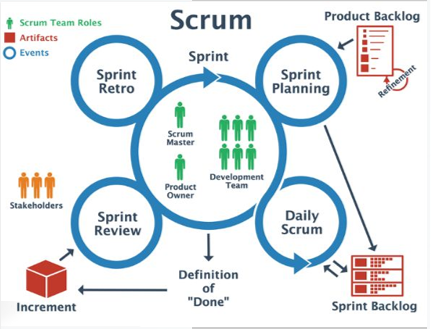
\includegraphics[width=0.8\textwidth]{include/image/scrum.png}
    \label{fig:scrum}
\end{figure}

\subparagraph{Product Owner}

Product Owner là người đại diện cho khách hàng hoặc các bên liên quan của dự án. Vai trò chính của Product Owner là xác định giá trị kinh doanh của sản phẩm và đảm bảo nhóm phát triển luôn tập trung vào những chức năng mang lại giá trị cao nhất.

Các nhiệm vụ chính của Product Owner bao gồm:

\begin{itemize}
\item Thu thập và làm rõ yêu cầu từ khách hàng.
\item Xây dựng và quản lý danh sách yêu cầu của sản phẩm.
\item Xác định mức độ ưu tiên của các chức năng.
\item Đưa ra quyết định liên quan đến phạm vi sản phẩm.
\item Tham gia đánh giá kết quả sau mỗi Sprint.
\end{itemize}

Product Owner đóng vai trò cầu nối giữa khách hàng và đội phát triển, đảm bảo sản phẩm cuối cùng đáp ứng đúng nhu cầu nghiệp vụ.

\subparagraph{Scrum Master}

Scrum Master là người chịu trách nhiệm đảm bảo nhóm làm việc đúng theo các nguyên tắc và quy trình Scrum.

Vai trò của Scrum Master không phải là quản lý trực tiếp các thành viên mà là hỗ trợ nhóm làm việc hiệu quả hơn bằng cách:

\begin{itemize}
\item Hướng dẫn nhóm áp dụng Scrum.
\item Tổ chức các cuộc họp Scrum.
\item Loại bỏ các trở ngại ảnh hưởng đến tiến độ công việc.
\item Hỗ trợ giao tiếp giữa các thành viên và các bên liên quan.
\item Thúc đẩy quá trình cải tiến liên tục trong nhóm.
\end{itemize}

Thông qua vai trò này, Scrum Master giúp nhóm duy trì năng suất và đảm bảo quá trình phát triển diễn ra ổn định.

\subparagraph{Development Team}

Development Team là nhóm chịu trách nhiệm trực tiếp xây dựng sản phẩm.

Tùy thuộc vào quy mô dự án, nhóm có thể bao gồm:

\begin{itemize}
\item Software Developer.
\item Frontend Developer.
\item Backend Developer.
\item Embedded Engineer.
\item Tester.
\item QA Engineer.
\item DevOps Engineer.
\end{itemize}

Đặc điểm của Development Team là tính tự quản (Self-organizing), nghĩa là các thành viên chủ động phân chia công việc, phối hợp với nhau để hoàn thành mục tiêu của Sprint thay vì phụ thuộc hoàn toàn vào cấp quản lý.

Mọi thành viên đều có trách nhiệm đóng góp vào việc hoàn thành sản phẩm và đảm bảo chất lượng của các chức năng được phát triển.

\subparagraph{Sprint}

Sprint là đơn vị thời gian cơ bản trong Scrum, thường kéo dài từ một đến bốn tuần.

Trong mỗi Sprint, nhóm phát triển sẽ thực hiện một tập hợp các công việc đã được lựa chọn trước đó và cố gắng hoàn thành chúng trong khoảng thời gian cố định.

Mỗi Sprint thường bao gồm các hoạt động:

\begin{itemize}
\item Sprint Planning.
\item Development.
\item Daily Scrum.
\item Sprint Review.
\item Sprint Retrospective.
\end{itemize}

Kết thúc Sprint, nhóm sẽ tạo ra một phiên bản sản phẩm có thể trình diễn hoặc triển khai thử nghiệm. Điều này giúp khách hàng đánh giá kết quả sớm và đưa ra phản hồi kịp thời.

\subparagraph{Product Backlog}

Product Backlog là danh sách toàn bộ các yêu cầu, chức năng, cải tiến hoặc sửa lỗi của sản phẩm.

Danh sách này được quản lý bởi Product Owner và luôn được cập nhật trong suốt vòng đời dự án.

Mỗi mục trong Product Backlog thường bao gồm:

\begin{itemize}
\item Mô tả yêu cầu.
\item Mức độ ưu tiên.
\item Giá trị nghiệp vụ.
\item Ước lượng khối lượng công việc.
\end{itemize}

Product Backlog đóng vai trò như nguồn công việc trung tâm của toàn bộ dự án và là cơ sở để lập kế hoạch cho các Sprint tiếp theo.

\subparagraph{Sprint Backlog}

Sprint Backlog là tập hợp các công việc được lựa chọn từ Product Backlog để thực hiện trong một Sprint cụ thể.

Trong cuộc họp Sprint Planning, Development Team cùng Product Owner sẽ lựa chọn các hạng mục phù hợp với năng lực thực hiện của nhóm trong khoảng thời gian Sprint.

Sprint Backlog giúp:

\begin{itemize}
\item Xác định rõ mục tiêu của Sprint.
\item Theo dõi tiến độ thực hiện công việc.
\item Đánh giá năng suất của nhóm phát triển.
\item Hỗ trợ quản lý và phân công công việc.
\end{itemize}

Trong quá trình thực hiện Sprint, Sprint Backlog có thể được cập nhật để phản ánh trạng thái thực tế của các công việc đang triển khai.

Thông qua mô hình Scrum, doanh nghiệp có thể quản lý công việc linh hoạt hơn, tăng khả năng phản hồi trước các thay đổi từ khách hàng và nâng cao hiệu quả phối hợp giữa các thành viên trong dự án.


\paragraph{6. Quy trình phối hợp với khách hàng}

Khách hàng là một trong những bên liên quan quan trọng nhất của dự án. Việc phối hợp hiệu quả giữa đội dự án và khách hàng giúp đảm bảo sản phẩm được phát triển đúng với nhu cầu thực tế và hạn chế các sai lệch trong quá trình triển khai.

Quy trình phối hợp thường bắt đầu từ giai đoạn khảo sát và thu thập yêu cầu. Trong giai đoạn này, các buổi họp trao đổi được tổ chức nhằm làm rõ nghiệp vụ, xác định các yêu cầu chức năng và phi chức năng của hệ thống. Các yêu cầu sau khi được phân tích sẽ được xác nhận lại với khách hàng để đảm bảo sự thống nhất giữa hai bên.

Trong quá trình thực hiện dự án, đội dự án thường xuyên báo cáo tiến độ, trình bày các kết quả đạt được và tiếp nhận phản hồi từ khách hàng. Các cuộc họp định kỳ giúp theo dõi tình trạng dự án, xử lý các vấn đề phát sinh và cập nhật các thay đổi cần thiết.

Đến giai đoạn nghiệm thu, khách hàng tham gia đánh giá sản phẩm dựa trên các tiêu chí đã được thống nhất từ trước. Kết quả nghiệm thu là cơ sở để thực hiện bàn giao và đưa hệ thống vào vận hành chính thức.

\paragraph{7. Quản lý thay đổi}

Trong thực tế triển khai dự án, các yêu cầu thay đổi là điều khó tránh khỏi do sự thay đổi của nhu cầu nghiệp vụ, quy trình vận hành hoặc các yếu tố khách quan khác. Vì vậy, việc quản lý thay đổi đóng vai trò quan trọng nhằm kiểm soát tác động của các thay đổi đến phạm vi, tiến độ, chi phí và chất lượng dự án.

Quy trình quản lý thay đổi thường bao gồm các bước tiếp nhận yêu cầu thay đổi, phân tích tác động, đánh giá tính khả thi, phê duyệt và triển khai thực hiện. Mọi thay đổi đều cần được ghi nhận và đánh giá trước khi đưa vào kế hoạch thực hiện nhằm tránh phát sinh các rủi ro không mong muốn.

Việc phân tích tác động giúp xác định mức độ ảnh hưởng của thay đổi đối với hệ thống hiện tại, nguồn lực dự án và các hạng mục công việc đang thực hiện. Sau khi được phê duyệt, các thay đổi sẽ được cập nhật vào kế hoạch dự án và thông báo đến các bên liên quan.

Thông qua quy trình quản lý thay đổi, doanh nghiệp có thể duy trì sự linh hoạt trong phát triển sản phẩm đồng thời vẫn đảm bảo khả năng kiểm soát dự án.

\paragraph{8. Quản lý rủi ro}

Quản lý rủi ro là hoạt động nhằm nhận diện, đánh giá và xây dựng các biện pháp ứng phó đối với những sự kiện có khả năng ảnh hưởng tiêu cực đến dự án.

Các rủi ro trong dự án công nghệ thông tin có thể đến từ nhiều nguồn khác nhau như thay đổi yêu cầu, thiếu hụt nguồn lực, sai sót kỹ thuật, chậm tiến độ, sự cố hạ tầng hoặc các yếu tố liên quan đến khách hàng.

Quy trình quản lý rủi ro thường bao gồm bốn bước chính:

\begin{enumerate}
    \item Nhận diện rủi ro.
    \item Phân tích mức độ ảnh hưởng và xác suất xảy ra.
    \item Xây dựng phương án giảm thiểu hoặc ứng phó.
    \item Theo dõi và cập nhật trạng thái rủi ro.
\end{enumerate}

Các rủi ro có mức độ ưu tiên cao cần được theo dõi thường xuyên và có kế hoạch xử lý cụ thể. Việc quản lý rủi ro chủ động giúp giảm thiểu tổn thất, hạn chế chậm tiến độ và nâng cao khả năng thành công của dự án.

\paragraph{9. Đảm bảo chất lượng}

Đảm bảo chất lượng (Quality Assurance - QA) là tập hợp các hoạt động nhằm bảo đảm sản phẩm và quy trình phát triển đáp ứng các tiêu chuẩn chất lượng đã đề ra.

Trong các dự án phần mềm, chất lượng không chỉ được đánh giá thông qua sản phẩm cuối cùng mà còn được kiểm soát trong toàn bộ vòng đời dự án. Các hoạt động đảm bảo chất lượng bao gồm rà soát tài liệu, kiểm tra việc tuân thủ quy trình, đánh giá kết quả kiểm thử và theo dõi các chỉ số chất lượng.

Bên cạnh QA, hoạt động kiểm soát chất lượng (Quality Control - QC) cũng được thực hiện nhằm phát hiện lỗi trong sản phẩm thông qua các hoạt động kiểm thử. Nếu QA tập trung vào việc phòng ngừa lỗi thì QC tập trung vào việc phát hiện và khắc phục lỗi trước khi sản phẩm được bàn giao cho khách hàng.

Việc kết hợp giữa QA và QC giúp nâng cao độ tin cậy của sản phẩm, giảm chi phí sửa lỗi và tăng mức độ hài lòng của khách hàng.

\paragraph{10. Hỗ trợ, triển khai và bàn giao}

Sau khi sản phẩm hoàn thành và vượt qua các vòng kiểm thử nội bộ, hệ thống sẽ được triển khai tại môi trường thực tế của khách hàng. Giai đoạn này bao gồm các hoạt động cài đặt, cấu hình, kiểm tra vận hành và đào tạo người sử dụng.

Để đảm bảo khách hàng có thể khai thác hiệu quả hệ thống, đội dự án chuẩn bị các tài liệu hướng dẫn sử dụng, tài liệu vận hành và các nội dung đào tạo liên quan. Các buổi hướng dẫn và chuyển giao kiến thức giúp người sử dụng nhanh chóng làm quen với hệ thống mới.

Sau khi hoàn tất triển khai, khách hàng tiến hành nghiệm thu dựa trên các tiêu chí đã được thống nhất trong giai đoạn xác định yêu cầu. Khi sản phẩm đáp ứng đầy đủ các điều kiện nghiệm thu, đội dự án thực hiện bàn giao hệ thống, tài liệu liên quan và các sản phẩm của dự án cho khách hàng.

Ngoài ra, doanh nghiệp còn cung cấp các dịch vụ hỗ trợ sau triển khai như xử lý sự cố, bảo hành, bảo trì và nâng cấp hệ thống nhằm đảm bảo hệ thống vận hành ổn định trong suốt quá trình sử dụng.

\subsubsection{Tổng kết tuần 1}